\chapter{Evaluation}
\label{chap:eval}

This section relates to the evaluation of various aspects of the project.  The Src researcher whom the project originally focused on was off on maternity leave for the duration of this phase of the project so it was not possible to perform any evaluations with them.

\section{First Evaluation}
\label{sec:eval1}

The first evaluation in the second phase of the project occurred in November 2013.  The user group was made up of two biologists:  one who had taken part in the first evaluation meeting and one person who had no knowledge of the project.

\subsection{User Group}

The original evaluation strategy was to use insight-based evaluation.  This is a technique proposed by Chris North~\cite{cn_vizbi}.  He proposed giving the program to non-expert users.  They then see what they can learn from visualisation.  These insights are then evaluated by an expert user.  The program can then be evaluated by the quality of insights that the non-expert users were able to glean from the visualisation.

As the domain expert was not available, insight based evaluation was not possible.  A more traditional approach had to be taken.  Before the evaluation  a typical scenario that a user might encounter was prepared.  The task was to open a file, annotate it and run the animation visualisation, and attach supporting documentation.  The task was prepared at two levels of instruction.  The first level was a paragraph of text that described what was to be done.  The second level was a step-by-step list of instructions to perform.  These tasks can found in Appendix~\ref{sec:task1}.  The user group was observed as they attempted the task and were offered assistance when required.  Afterwards the user group was given a questionnaire to fill in about their experience. After filling in the questionnaire there was a discussion on their answers and any further thoughts that they had.  The questionnaire and results can seen in Appendix~\ref{sec:qs}

The task was prepared at two levels to try and gauge how easy the program is to use.  The users were first presented with the textual description and if they had been unable to complete the task with this then they would have been given the step-by-step instructions instead.  The users were able to complete the task from the textual description alone.  This is a good sign that the new tool is usable.

Some issues were encountered:

\begin{itemize}
\item The users were unfamiliar with \texttt{MacOS} -- Both users were unable to locate the menu bar as it is not attached to the program as in Windows.  Future evaluations were intended to be performed using Windows.  There were, however, issues in setting up the program on Windows.  Future evaluations happened on \texttt{MacOS}.
\item The users were unclear as to what was going to happen when annotating.  When annotating the graph with an arrow the user had to click twice to place it but there was no indication of this, nor was it clear to them which way the arrow would be drawn.  This was subsequently fixed. Different cursors are used to give feedback to the user that they should click, and rather than just relying on two clicks with no information as to where the arrow is going to point, after the first click (which places the tail of the arrow) an arrow is drawn that follows the cursor until the second click placing the annotation.
\item Lack of ability to edit, move, or delete annotations. Once an annotation was placed it was there permanently.  The ability to edit annotations was always planned, but had not been implemented in time.  But the amount of frustration it gave the users was very high.  It was a principle in all three of Norman~\cite{normsev}, Neilson~\cite{neilten} and Schniederman's~\cite{shgold} lists that a user should be able to fix mistakes.  Since the evaluation, editing and deleting of annotations have been implemented.  This means any mistakes can be corrected.
\item Initially the users were confused by what all the buttons on the \texttt{matplotlib} toolbar did.  After discovering the tooltips, and seeing what effect the buttons had, they were comfortable with them.  If a user were to do something they did not intend they are able to undo it. All the \texttt{matplotlib} built-in buttons on the toolbar can be undone and redone from the toolbar.  Any buttons implemented for this tool are covered by the undo and redo functionality implemented across the whole program.  Being able to recover from their actions on the toolbar means no hindrance to discovery and so needs no further action.  It would be desirable to have the two undo methods unified but a way to do this could not be found.
\item The users were confused by some of the terminology.  In particular they could not distinguish between ``save graph'' and ``save model''. These items in the menu have now been grouped more carefully to help the user distinguish them.  A related issue was worrying that ``save graph'' was going to override the results file.  To rectify this the menu items that create new files have been renamed ``export ...''.
\item The users struggled to start a new session.  When asked for a title they did not know what the title was going to be used for.  When trying to add files, rather than use the add files button in the dialogue, they tried to use the file menu.  Having two routes into the visualisation seemed to be confusing them.  Now the file menu open file has been removed.  To create a visualisation the user has to go through the new session wizard.
\item When placing species in the cell one of the users did not understand what they were being asked to do.  One of the users did understand.  To fix this user input has been removed from the process.  The species locations are parsed automatically from the model.  This has required the model file to be added to the session by the user.
\item They liked the animation feature and thought it would be very useful. One of the users did their PhD in transport and expressed a desire to have had this feature during the PhD.  They did feel that it wouldn't be useful directly for papers, but that it would be useful when deciding what to include in a paper.
\item One of the users asked if there was a map of the cell.  When presented with the model visualisation they thought that it did look nice, but they were unsure of its usefulness.  The model viewing has since been merged into the animation visualisation.
\item The results from the questionnaire indicated that both users thought the tool's appearance was good.  The tool was average in difficulty to use -- neither easy nor difficult. The annotation buttons on the toolbar were clear as to what they did. It was obvious how to attach supporting files.  Both users thought that it is very useful to attach files to the session so that they can be easily emailed to a colleague.  They thought it would be useful to have the graph automatically annotated, but they wanted to the ability to disable any automatic annotations.
\end{itemize}

\subsection{Personal Evaluation}

At this stage in the development the program was in a state where some existing functionality had been broken.  This had not been noticed during development.  This highlighted architectural flaws in the code.  There were multiple paths through the program that data was taking.  Code was also duplicated across the program.  The majority of these bugs have since been ironed out and the duplicated code removed. The code has a better architecture.  At the time of the evaluation with the users not all the features could be tested with them -- mainly the plot preferences dialogue.  These features have since been fixed and they were evaluated by the users at the next meeting.

Having the users use the program also highlighted a number of usability problems: menus being badly organised and named, features such as annotation relied on assumed knowledge to work them.  All this created an unfriendly environment for the user.  This was due to losing sight of the need for usability during development and when testing new features not removing the knowledge of the code from my mind.  After this evaluation the three lists of usability~\cite{shgold}\cite{normsev}\cite{neilten} were focused on again and the code was reviewed and the principles applied.

The positive feedback on animation and annotation, two of the core new features, was excellent validation of the new work.

\section{Evaluation 2 - Start of Second Semester}
\label{sec:eval2}

The second evaluation in the second phase of the project occurred in February 2014.  There were two evaluations this time.  One with the same group of biologists as before and another with an Informatics researcher who uses Bio-PEPA.

Since the previous evaluation work had been done to fix the issues encountered and two new features had been added: annotation of the animation and data normalisation and export.

\subsection{User Group}

As with the first evaluation a task was prepared at two levels of instruction.  The task can be seen in Appendix~\ref{sec:task2}.  Afterwards the users were given a questionnaire to fill in.  The questionnaire and results can be seen in Appendix~\ref{sec:qs}.  They were also given a chance to use the program without following a task, giving them a chance to explore.  Again, after the questionnaire a discussion was held.

The findings of the evaluation were as follows:

\begin{itemize}
\item There were inconsistencies in the text within the tool that is intended to guide users.  This did not appear to cause confusion, but it was noticed by both of the users.  This was fixed.  All the user facing text in the project was checked and changed if inconsistent.
\item The users kept trying to drag annotations on the graph after creation. The users wanted to be able to drag the annotation to a new position to fine-tune the position.  They attempted to do this by left clicking on the annotation and dragging it.  This issue has not been solved.  Currently if the user places an annotation in the wrong location they can delete the annotation and put a new one in the correct place.  For the user this is not the most desirable solution, but it was felt that the time could be better spent in other areas of the project.  This would, hopefully, be implemented in future work.
\item The users found the new model visualisation much more informative.  This is a positive as the reason for implementing model visualisation was to help the users understand what happens in the model more.  The users did however think that adding in labels of the compartments would be useful as they may not be familiar with the model.  The labelling of compartments has since been implemented.
\item The users found the task to be easy to complete.  This is a good result.  The tool needs to be easy to use.  They did not give full marks for ease, so there was still room for improvement.
\item The users found it much easier to start a new session using the wizard.  This was a task they had struggled with during the previous evaluations.  There were still aspects that they did not discover such as being able to select multiple files.  Guidance text has since been added to the wizard pages.
\item The users indicated that they found annotating animations easy and intuitive.  This is positive.  It is a new feature and the users indicated little need for change.
\item The users uncovered some bugs in the system.  The bugs included: not all types of annotations could be placed on the plot and the colours of the cell segments not being updated after changing the colour of the line.  All bugs discovered have since been fixed.
\item The users were very much in favour of being able to use plots as queries.  This provided justification for pursuing this as a project goal.
\item The users were very much in favour of being able to collaborate in real time. This provided justification for pursuing this as a project goal.
\item The users found it easy to normalise and export the data and indicated that they thought it would be a useful feature to have.
\item The users were pleased by the addition of undo functionality.  They appeared to be much more willing to make mistakes knowing that they could undo their mistakes.
\item The users were pleased that since the last evaluation the ability to modify and delete annotations had been added.
\end{itemize}

\subsection{Bio-PEPA Developer}

The evaluation with the Bio-PEPA developer was similar to the evaluation with the user group.  The developer was given the same task and after performing the task there was a discussion about their performance and their feelings about the tool.

\begin{itemize}
\item It was not clear to the user what the new model visualisation was displaying.  This has been solved by adding text to the model visualisation page explaining what the user is seeing.
\item The user uncovered a bug in how annotations are rendered when the graph is viewed with the data normalised.  The problem and the solution are discussed in Section~\ref{sec:annotation_graph}.
\end{itemize}

\subsection{Personal Evaluation}

The results from this evaluation were positive.  The users seemed much more comfortable using the tool.  This was hopefully down to the efforts made to improve the usability.  There were still too many bugs being discovered by the users.  This was addressed by spending a significant amount of time on tracking down and fixing bugs.  The positive reception to the ideas for plots as queries and real time collaboration led to them being added as project goals.

\section{Evaluation 3 - End of Second Semester}
\label{sec:eval3}

The third and final evaluation in the second phase of the project occurred in March 2014.  There were two evaluations this time.  These were the same as the previous evaluation: the user group and an Informatics researcher who uses Bio-PEPA.  Given that this was the final evaluation a further focus was placed on evaluating the users' preferences between this new tool and the Eclipse plugin.

Since the previous evaluation a sizeable amount of work had gone into improving the stability.  The new features that had been added were plots as queries and real time collaboration.  These could not be evaluated by the users. Plots as queries could not be evaluated as it has not been tied into the \ac{UI}.  Real time collaboration could not be evaluated with the users as it would have required another laptop.  The layout of the program had changed and this was tested by the users.

\subsection{User Group}

Like the other evaluations the users were given a task to complete.  The task can be found in Appendix~\ref{sec:task2}. Afterwards there was a questionnaire and a discussion.  The questionnaire and results can be found in Appendix~\ref{sec:qs}

The findings were as follows:

\begin{itemize}
\item The users liked the appearance of the tool.  Since the previous evaluation significant effort had been placed on making the user interface more aesthetically pleasing.  The users strongly preferred the new \ac{UI}.  This justifies the effort put into the \ac{UI}.
\item The users indicated that they found the task easy to complete.  They were not confused by the new layout.
\item Both users indicated that they would rather use this than the Eclipse plugin.  They did both give the proviso that they have zero experience with the Eclipse plugin beyond what they were shown in the evaluation.  In the evaluation they were shown an example of a graph that the plugin generated.  Both users preferring to use this new tool rather than the Eclipse plugin was excellent validation of the project aims.
\item Both users were unable to give feedback about features they felt were missing or features they would like to see as they had not spent enough time with the tool.  Further evaluation time with ethnographic studies would be required for this.
\item When creating an animation annotation the users set the duration to be after time zero.  They were confused afterwards as to why the annotation was not immediately visible on the cell.  It had been hoped that it would be obvious that if the current clock was not in the duration of the annotation then it would not be visible.  This was solved by updating the clock to be the start time of the annotation being created. This means it is always visible to the user that an annotation has been successfully placed.
\item The slowness of the tool caused the users some frustration.  They would frequently want to perform the next action, while the program was still trying to update the visualisations.  This is a problem that has been discovered with matplotlib -- it is quite slow.  This has not been resolved.
\item The users found the model visualisation more helpful now that labels had been added.
\item The users appreciated the addition of helper text to various parts of the \ac{UI}.
\end{itemize}

\subsection{Bio-PEPA developer}

The user was presented with the same task as the user group.  The task can be found in Appendix~\ref{sec:task2}.  After completing the task they were asked to fill in a questionnaire.  After filling in the questionnaire there was a discussion about their performance.  The questionnaire and results can found in Appendix~\ref{sec:qs}

\begin{itemize}
\item The user felt that the appearance of the tool was adequate, although they far preferred the new \ac{UI}.  They did not rate the appearance as highly as the biologist users.  They were unable to explain why they had not scored it higher in appearance.  They said they would like to see more headings on the different parts of the \ac{UI} in the future.  This would be resolved if development were to continue.
\item The user indicated that they found it difficult to complete the task.  In previous evaluations they did not find it as difficult.  This was due to the lag in the \ac{UI} when updating the visualisations.
\item When asked whether they would use this tool instead of the Eclipse plugin the user said it depended on what task they were trying to perform.  If they were preparing images for publication they would use this new tool.  If they were just analysing the model they would use the Eclipse plugin.  This was to be expected.  Future work would hopefully be done to integrate the workflow between the Eclipse plugin and this new tool.  It important to note that this user is not the target user.  The biologists are the target audience, their preferences are more important for the evaluation.
\item The user would have liked to see the model visualisation being able to handle models that were not necessarily hierarchical.  This would hopefully be looked into for future work.
\item The user would have liked to have been able to evaluate the tool with more models which covered a variety of scenarios.  This was not possible in this evaluation strategy. A direction for future evaluations would be ethnographic studies.
\item The user did not discover the context menu for annotations, they had to be told about this.  No solution has been found to make this feature more discoverable.
\item The user uncovered an issue that made it very difficult to right click on text or circle annotations.  These annotation types use point to point Euclidean distance.  This meant that the user had to right click near the start point of the annotation.  This start point is not obvious at all.  This problem has not been fixed.  For the circle annotation it would be possible to use the equation of a circle to check if the mouse click is near any point in the circle.  For the text annotation it would be very difficult to solve the problem as the text annotation has no concept of its size.
\end{itemize}

\subsection{Personal Evaluation}

The final evaluation definitely revealed that the project has had positive outcomes.  The users were all in favour of the project and would use it in their workflow.  The reception of the new \ac{UI} layout was very positive.  Fewer bugs were discovered than in previous evaluations. There are still usability flaws and further, more in depth evaluation is, ideally, needed.

\subsection{Validity of These Results}
The findings from the user evaluations should be taken with a pinch of salt.  The tool was evaluated by a small number of users.  They did not spend a significant amount of time using the tool.  This limits the meaningfulness of the findings.  There were not enough biologists or potential users available to perform a significant number of evaluations.

In particular the user's opinions on whether the tool was easy to use or not, and their ease with completing the task are not independent between evaluations.  Asking a set of users to repeatedly use a tool and perform a task will lead to them becoming more familiar with the tool and the task and future attempts will be easier for them.  Their opinion on ease of use may be built on the experience across evaluations.  This is an unavoidable problem when evaluating multiple times with the same set of users.  There were not enough biologists available to use different users in each evaluation.

The users were also not able to spend a significant amount of time using the tool.  The evaluations performed were a good initial set of evaluations and uncovered a lot of the usability flaws.  An ethnographic study would involve users in their natural environment using the tool over a long period of time.  This would be a very in-depth and time consuming evaluation technique.

\section{Self Evaluation}
The feedback from potential users was a very important part of the evaluation.  There are other important aspects of the evaluation.  Metrics exist for evaluating the quality of a \ac{UI} and its usability.  The quality of the visualisations must also be measured.  The performance must be evaluated.  These aspects of the evaluation can be found in this section.

\subsection{Evaluation of the Architecture}

In Section~\ref{sec:architecture}, the architecture of the tool is discussed.  During the second phase of development the program was given an architecture similar to \ac{MVC}, but with little distinction between the view and the controller.  This was a step in the right direction.  The program would, however, have a much better architecture if it was fully \ac{MVC}.  This would have made the implementation of real time collaboration much easier. Having a \ac{MVC} architecture would also make future development easier.  This is discussed in Section~\ref{sec:conc_architect}.

The program architecture suffered towards the end of development when real time collaboration was added as a feature.  The code was not fully \ac{MVC} and collaboration had not been a potential feature during the architectural design.  The collaboration feature introduced an entirely new route through the program.  Due to the project time table there was no time to refactor the architecture.  This led to collaboration being somewhat bolted on.  Some of the functionality necessary for real time collaboration was put into the singleton object.  This was less than ideal.  The better solution would have been to create a controller and put the functionality there instead.  This was not possible due to time constraints.
%Does this contradict what was said in implementation?

\subsection{Meeting HCI Principles}
\label{sec:principles}

Norman~\cite{normsev}, Shneiderman~\cite{shgold} and Neilson~\cite{neilten} each have a set of principles for \ac{UI} design.  Whilst planning this project it was decided that these principles would form a useful evaluation metric.  The principles and how this project meets or does not meet them are detailed in this section.  There are overlaps between the sets of principles.  If there is an overlap it has been indicated.

\paragraph*{Striving for consistency} is a principle in all three lists.  It suggests that platform conventions should be followed, similar actions should have similar effects and terminology should not change across the \ac{UI}.  Conforming to platform conventions has not been strictly followed in this project.  The intention was to be cross platform.  An attempt was made, with respect to the menubar, to follow \texttt{MacOS} guidelines.  However there are not enough menu options to make this obvious.  Terminology has been kept as consistent as possible across the \ac{UI}.  Efforts were made for similar actions to elicit similar results, however this was not always successful.  There is a big inconsistency between built-in \texttt{matplotlib} functionality and functionality implemented by this tool.  For example, there are two different undo mechanisms.

\paragraph*{Enabling shortcuts} is principle in Shneiderman's and Neilson's principles.  Shortcuts are there for expert users to save them time.  There are standard shortcuts, i.e. \texttt{Ctrl-S} for save.  Standard shortcuts can be considered user friendly.  Custom shortcuts are not user friendly, but they enable an experienced user to speed up their workflow.  Standard and custom shortcuts were implemented in this tool according to \texttt{wxPython} specification.

\paragraph*{Offering informative feedback} is in all three lists of principles.  This is so the user is kept aware of system state.  They should be receiving feedback from every action. Feedback was, sometimes, a natural byproduct of the features; for example, when loading a results file the feedback that the load operation has been successful is that a graph appears on the screen. If the graph does not appear then something has gone wrong.  Other forms of feedback have been explicitly added.  These include:
\begin{itemize}
\item When adding annotations the cursor changes to indicate to the user that they can interact with the graph in a different way.
\item The title bar text changes to display ``unsaved'' when the user makes a change and then changes back to ``saved'' when a successful save has been performed.
\end{itemize}

\paragraph*{Designing dialogues to yield closure} is a principle in Shneiderman's principles.  It calls for encapsulating sequences of actions with dialogues.  Finishing the dialogues allows the user to clear their mind.  The new tool makes significant use of dialogues to improve the user experience.

\paragraph*{Offering simple error handling} is a principle of Shneiderman's and Neilson's principles.  The user should be prevented from arriving at an error state.  This was a problem throughout the project.  During development, any error states that were found were removed. This was done through exception catching and more defensive programming.  If new error states were discovered the same techniques would be applied.  If the user performs an action they did not mean to, which could be classed as an error, they are able to undo it.

\paragraph*{Permitting easy reversal of actions} is a principle in Shneiderman's and Neilson's lists.  It is intended to give users a way of escaping error states by reverting to previously working states.  This has been implemented through undo and redo.  Copies of the data dictionary are pushed and popped onto the stack.  Copies are pushed onto the undo stack on any atomic change the user makes.  This gives the user a full session history to go back through.

\paragraph*{Supporting internal locus of control} is one of Shneiderman's principles.  It calls for making the user feel in control of the system and having the user instigate actions rather than respond to actions.  The user is the instigator of all actions in the tool.  The sense of control will be lost when collaborating as actions will be performed that they did not instigate.  This is unavoidable and is mitigated by the fact that the users have to instigate a collaborative session.

\paragraph*{Reducing short-term memory load} is a principle in Shneiderman's and Neilson's lists.  It calls for keeping \acp{UI} simple.  It is important that users should be able to \textit{recognize} what action needs to be performed, not \textit{remembering} what action has to be performed.  This has been done by clearly and effectively labelling \ac{UI} elements and by having a shallow structure.  The user is not forced to go through deep menus and dialogues to perform actions.  When implementing \acp{UI} that are optimised for recognition it is important not to end up in a Norman door situation~\cite{design_of_things}[p.87].  A Norman door is a door that has been particularly poorly designed and is labelled push or pull, rather than made clear through the design of the door.  Some minor Norman door situations have found their way into the project.  The most obvious one is in the session wizard on the results file selector page.  The user is able to select multiple files.  During evaluations the user did not discover this, so helper text was added telling the user that multiple files can be selected.  It had been assumed to be obvious, as it is a feature in many programs that you can select multiple files.

\paragraph*{Constraining the user} is one of Norman's principles.  It suggests finding ways to restrict what actions a user can perform during use of the program.  This can be used to help guide the user through the program.  This has been accomplished in this project through the use of wizards and by enabling and disabling various \ac{UI} elements.

The first evaluation of the second phase of the project unearthed that the users struggled to choose the correct action as there were multiple ways of performing the same action that had slightly different use cases.  For example, at one point results files could be added via two different menu items.  They were not constrained enough.  These multiple paths have been removed. Now there is only one way, initially, to open results files.  To help guide the user further, \ac{UI} elements are enabled and disabled as appropriate.  Now when the program is first loaded the only action a user can perform is to load a session or start a new session, or join a session.  Afterwards other \ac{UI} elements are enabled to allow the user to start using the tool effectively.  This guides the user through their use of the program.

To help guide the user when they first use the program a session wizard is created.  This replaced a series of separate menu items that the user previously had to navigate. The new session wizard would typically be the entry route in the first time a user runs the program.  It was therefore important that it helped them understand what it is they are doing.  The process of setting up the session should also be as easy as possible so that the user does not dislike the prospect of using the program.  The session wizard can be seen in Figure~\ref{fig:session_wizard}.

\paragraph*{Providing mappings to the real world} is one of Norman's and Neilson's principles.  It suggests that the program should `speak the user's language' and use words, phrases and concepts that are familiar to them.  The cell cross-section animations are an example of that in this program.  It maps the results data into a form that is more familiar to biologists.

\paragraph*{Making use of affordances} is one of Norman's principles.  Is calls for using visual clues to help guide the user.  Different mouse cursors were used to indicate to the user that different functionality could be performed.  The principle of affordances in linked to the principle of reducing short term memory load, as affordances enable recognition.

\paragraph*{Having an aesthetic and minimalistic design} is one of Neilson's principles.  It calls for not having unnecessary information in the \ac{UI} as it competes with the relevant information for the user's attention.  This is quite a subjective criteria, however the user feedback would seem to indicate that it has been met.

\paragraph*{Providing help and documentation} is one of Neilson's principles.  It calls for having documentation available for the user in case they need it.  This project has no user documentation.  This is because the time that could have spent writing documentation was better spent implementing innovative features.  If time was not a factor in the project then user documentation would have been written.

The new tool has been quite successful at meeting these principles.  We can consider therefore that it has a good interface, with room for improvement.  The area that most needs improving is enabling recognition without the use of text explaining to the user what to do.  More use should be made of visual cues.  This also saves the user having to read lots of text.

\subsection{Visualisation Quality}

Edward Tufte's The Visual Display of Quantitative Information~\cite{tufte} is a seminal work in the field of data visualisation.  In his book Tufte outlined a number of metrics that can be used to evaluate the quality of a visualisation.  Given that this project is primarily a data visualisation tool it is important that visualisations are of a high quality.  Tufte's metrics have been used for evaluating the quality of the visualisations in this project.

Tufte provides a checklist for graphical excellence~\cite{tufte}[p.13].  These are set of points that describe what a visualisation should be.  They therefore can be a useful evaluation metric for visualisations.

According Tufte graphical displays should:
\begin{itemize}
\item Display the data.  This was accomplished in the new tool.
\item Make the user think about the visualisation, not how it was created.  This is a very subjective metric.  It is believed to be more relevant to more complex infographics rather than graphs.
\item Avoid distorting the data.  This was accomplished in the new tool.  Data is not distorted.  The displaying of the normalised data, in some circumstances, fall foul of this guideline.  When the data was normalised some plots appeared to grow in size.  The shape was preserved, but the scale was changed.  This gives an appearance of a larger change.  This is unavoidable when normalising data.  It is also a user initiated action, it is not hidden from them.
\item Present many numbers in a small space.  This was accomplished.  Thousands of data points are plotted on the graph.
\item Make large datasets coherent.  This is believed to have been accomplished, the data is plotted in line graph form, which is, typically, easy to interpret.  One of the aims of the project was to make the datasets coherent for those who are not comfortable with traditional graphs.  For these users, the cell level animation makes the data coherent.
\item Encourage the eye to compare different pieces of data.  This is another metric that seems more relevant to complex infographics.  It was accomplished in this tool.  Multiple species can be plotted on the same graph.  It is natural to compare the data.
\item Reveal the data at several levels of detail.  This was accomplished.
We have the traditional graphs and cell cross-sections.  The graph provides detail on the structure and the cell cross-sections provide a broader overview of the data.
\item Serve a clear purpose.  This tool does have a clear purpose. The goal of the project was to ``Visualise the results of dynamic time-series models of intra-cellular behaviour based on biochemical reactions".  This goal has been met.  This is discussed further in Section~\ref{sec:met_goal}.
\item Be closely integrated with statistical and verbal descriptions of the dataset.  The ability to add annotations to the visualisations accomplishes this goal.  The annotations provide the verbal description and the the graphs provide the statistical description.
\end{itemize}

We can see that the tool has met most of these guidelines.  This indicates that the visualisations offered are good quality visualisations.

\paragraph*{The Golden Ratio} is suggested by Tufte as the proportion to use for the size of a graph~\cite{tufte}[p.189].  The golden ratio is also believed to be aesthetically pleasing to humans.  The aspect ratio of the graph in the tool approximates the golden ratio.

\paragraph*{Data Ink} is a metric for determining how much redundant information is in a visualisation~\cite{tufte}[p.93].  This has not been formally calculated as the definition of redundant information is not well defined, especially with respect to annotations.  The concept of reducing redundant information is still an important aspect and was taken into consideration.  There is no unnecessary decoration on the graphics.  Only relevant information is displayed.

\paragraph*{Lie Factor} is a metric for whether a visualisation is misrepresenting the information~\cite{tufte}[p.57].  It is calculated by $\frac{\text{size of effect in graph}}{\text{size of effect in data}}$.  This was identified as an evaluation metric because correctly representing the data is vital.  The visualisations available in this tool do not misrepresent data.  The visualisations are plotting the data.  Lie factor is more of an issue in fancier graphics.  The displaying of the normalised data, in some circumstances, fall foul of this guideline.  When the data was normalised some plots appeared to grow in size.  The shape was preserved, but the scale was changed.  This gives an appearance of a larger change.  This is unavoidable when normalising data.  It is also a user initiated action, it is not hidden from them.

\subsection{Finished Product}

As well as evaluating the program as a whole, it is necessary to evaluate the major components.

\subsubsection{The User Interface}

Figure~\ref{fig:main_ui} shows the main screen of the \ac{UI} at the end of the development phase.  Figure~\ref{fig:old_ui} shows the previous version of the \ac{UI}.  The widgets have, now, been placed in a more organised and consistent manner.  This style has been continued through the rest of the screens in the \ac{UI}.  A heading to the legend panel has been added.  This indicates to the user from the start where the legend will be placed.  It has also been much more prominent in an effort to draw the users attention to it.  The legend panel has been moved over to the right hand side to remove the boxed in feeling that the previous \ac{UI} gave.

\begin{figure}[h!]
    \centering
    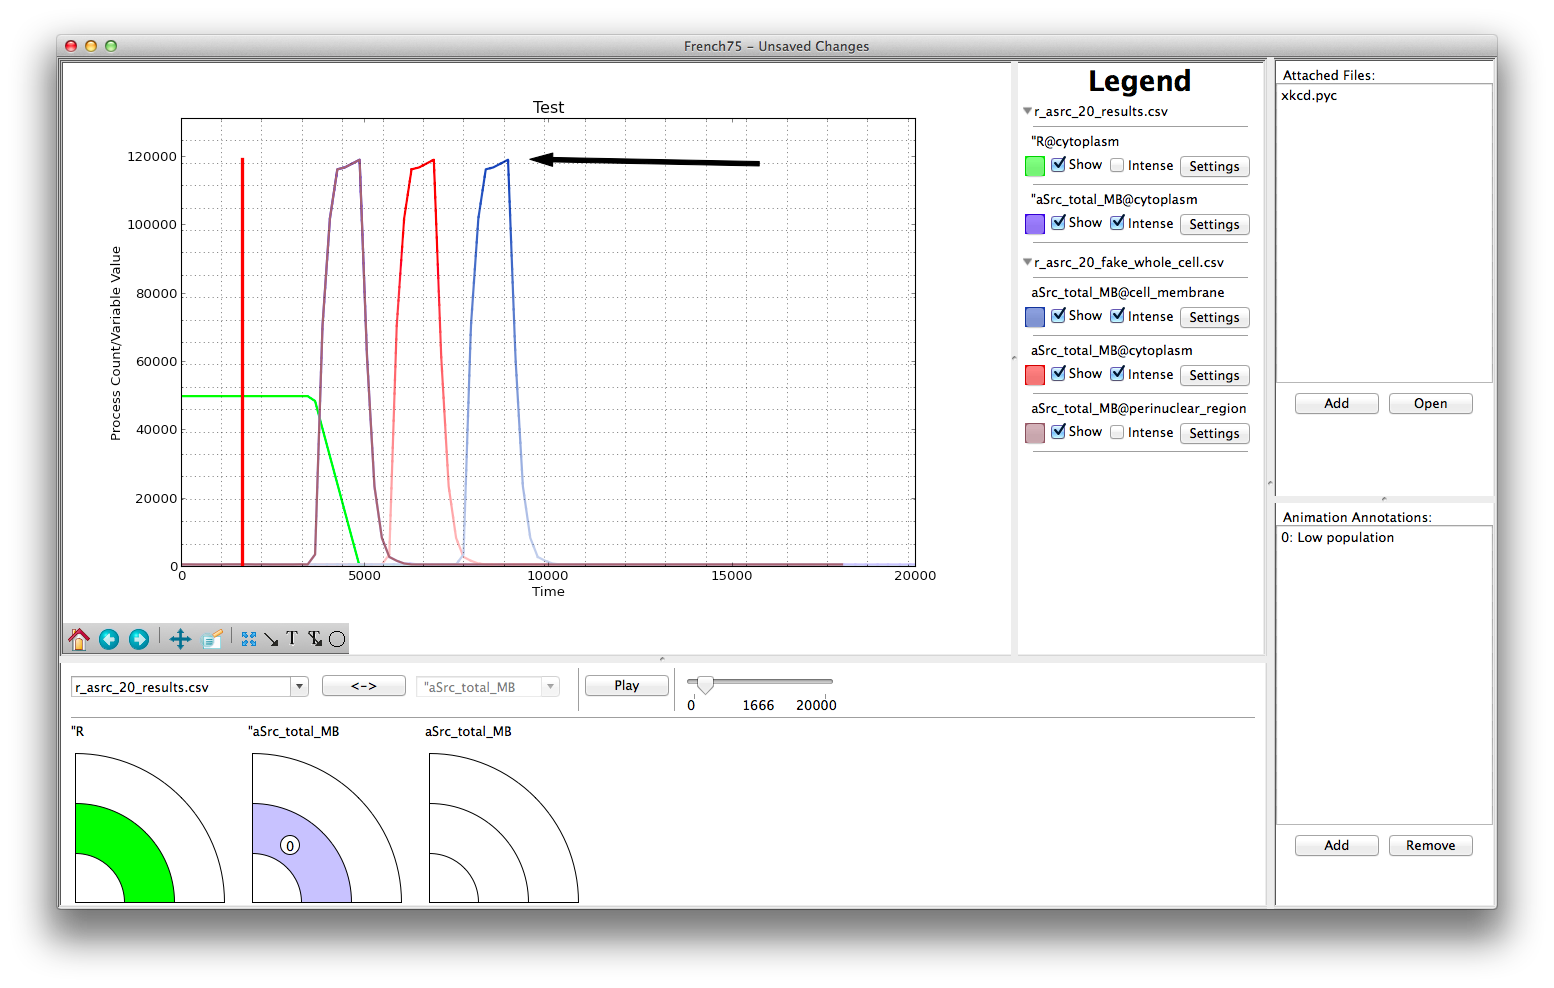
\includegraphics[width=\textwidth]{images/main_ui.png}
    \caption{Final \ac{UI}}
    \label{fig:main_ui}
\end{figure}

\begin{figure}[h!]
    \centering
    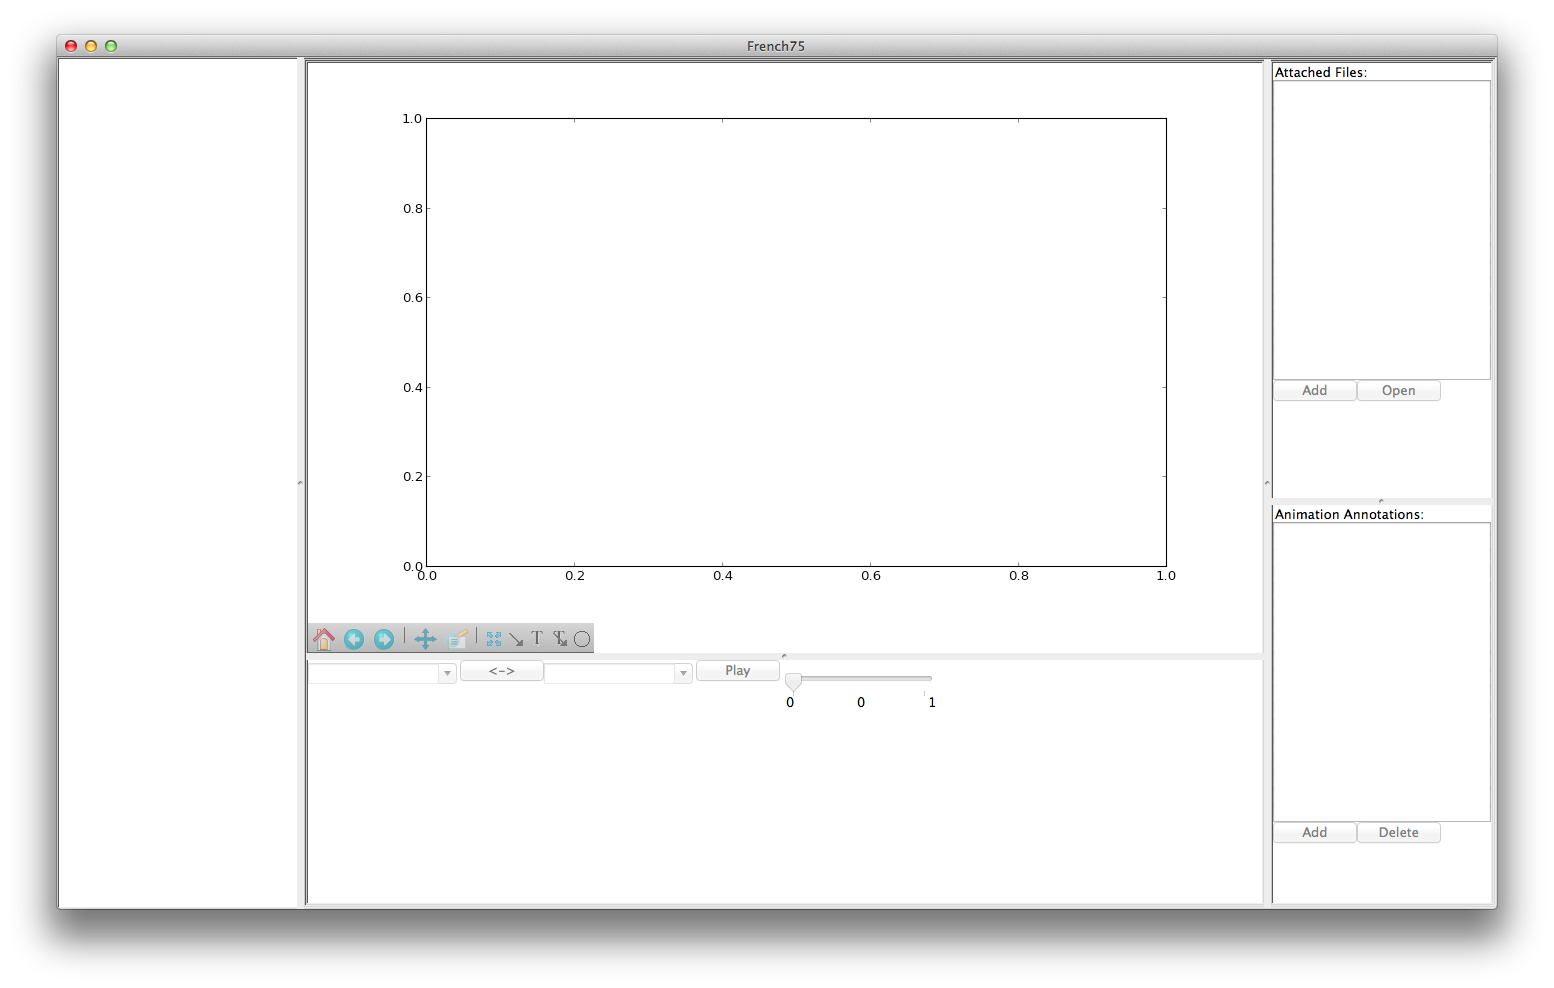
\includegraphics[width=\textwidth]{images/old_ui.png}
    \caption{Earlier \ac{UI}}
    \label{fig:old_ui}
\end{figure}

Figures~\ref{fig:add_anime_annotation}~and~\ref{fig:line_settings} show the dialogues that are presented to the user for creating an animation annotation and changing the preferences of a line.  There is a consistent style to the dialogues to help the user feel comfortable.  In both dialogues related widgets are grouped together.  It was not felt necessary to use wizards for these functions.  Wizards imply a set of steps that need to be followed.  For the plot preferences dialogue there is no concept of order.  For the annotation dialogue there are not enough steps to warrant a wizard.  The plot preferences dialogue in Figure~\ref{fig:plot_prefs_dialogue} spawns another dialogue when the user initiates a change colour action.  The spawned dialogue can be seen in Figure~\ref{fig:colour_picker}.  This is one of the most user unfriendly aspects of the entire \ac{UI}.  Whether you choose a new colour or not, the only way to exit the dialogue is by pressing the red close button.  This is a standard cancel action.  It does not inform the user that their action is going to be successful.  This confused all users.  This is a default dialogue provided by \texttt{wxPython}.  Ideally it would have been fixed, but there was not time.

\begin{figure}[h!]
    \centering
    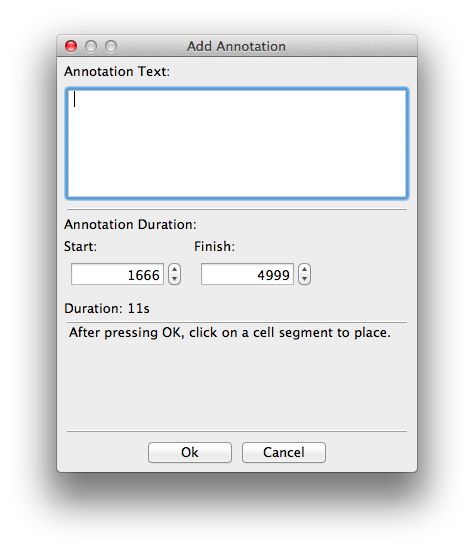
\includegraphics[width=0.5\textwidth]{images/add_annotation_dialogue.png}
    \caption{Add animation annotation dialogue}
    \label{fig:add_anime_annotation}
\end{figure}

\begin{figure}[h!]
    \centering
    \begin{subfigure}[b]{0.6\textwidth}
        \centering
        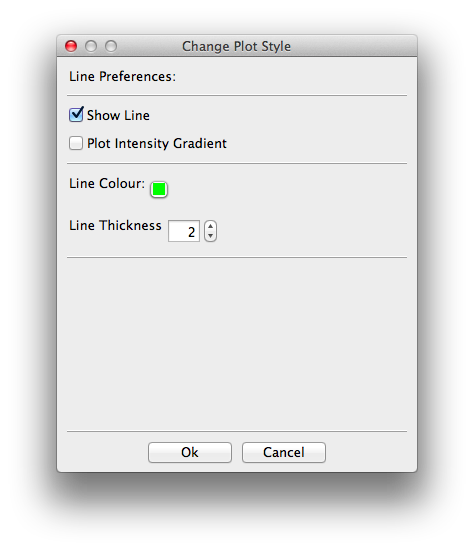
\includegraphics[width=\textwidth]{images/plot_preferences_dialogue.png}
        \caption{Line preferences dialogue}
        \label{fig:plot_prefs_dialogue}
    \end{subfigure}
    \begin{subfigure}[b]{0.3\textwidth}
        \centering
        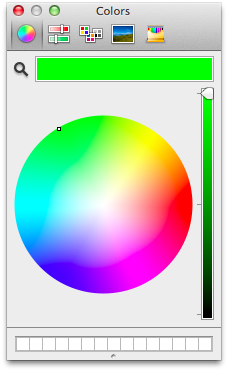
\includegraphics[width=\textwidth]{images/colour_selector.png}
        \caption{Colour chooser dialogue}
        \label{fig:colour_picker}
    \end{subfigure}
    \caption{Line settings dialogues.}
    \label{fig:line_settings}
\end{figure}

Wizards were used to guide the user through the process of setting up a new session.  The wizard can be seen in Figure~\ref{fig:session_wizard}.  A predecessor of the wizard can be seen in Figure~\ref{fig:old_session_dialogue}.  The old dialogue was not user friendly.  The user is presented with a long list of boxes that need to be filled.  This is overwhelming to a user.  It is also quite ugly.  The new session wizard fixed this.  The wizard follows the style of the other \ac{UI} screens, providing the user with a consistent experience.  Having different pages in the wizard for each step of the new session process means that the user does not need to remember the whole process.  They can focus on the current step.

\begin{figure}[h!]
    \centering
    \begin{subfigure}[b]{0.4\textwidth}
        \centering
        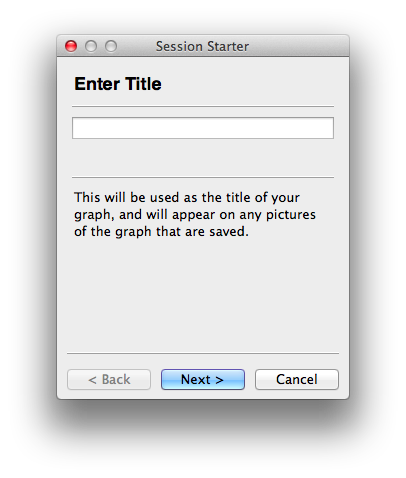
\includegraphics[width=\textwidth]{images/wizard_page_1.png}
        \caption{Wizard title chooser page}
        \label{fig:page_1}
    \end{subfigure}
    \begin{subfigure}[b]{0.4\textwidth}
        \centering
        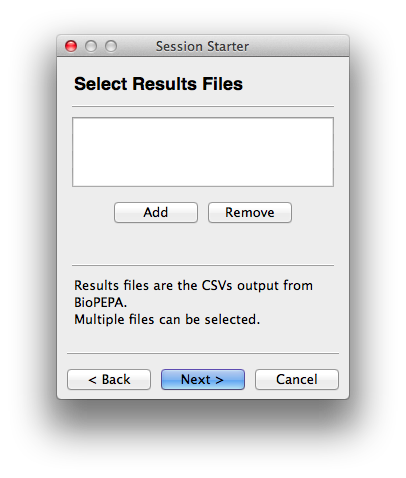
\includegraphics[width=\textwidth]{images/wizard_page_2.png}
        \caption{Wizard results selector page}
        \label{fig:page_2}
    \end{subfigure}

    \begin{subfigure}[b]{0.4\textwidth}
        \centering
        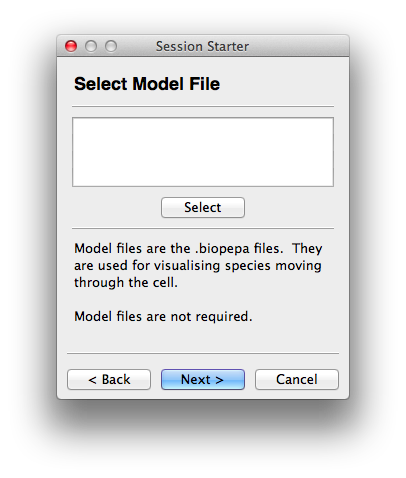
\includegraphics[width=\textwidth]{images/wizard_page_3.png}
        \caption{Wizard model selector page}
        \label{fig:page_3}
    \end{subfigure}
    \begin{subfigure}[b]{0.4\textwidth}
        \centering
        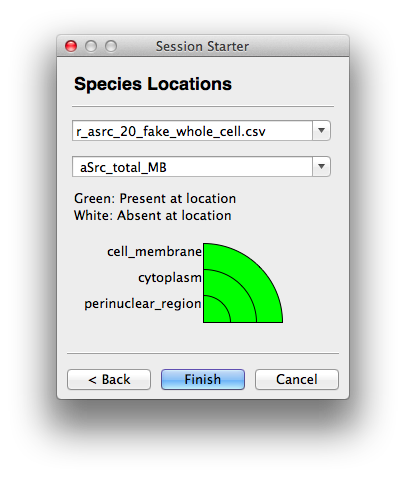
\includegraphics[width=\textwidth]{images/wizard_page_4.png}
        \caption{Wizard model viewing page}
        \label{fig:page_4}
    \end{subfigure}
    \caption{The session wizard that guides a user when setting up a session.}
    \label{fig:session_wizard}
\end{figure}

Form validators are used on the title fields and results fields.  The validators ensure that a title and at least one results file are included.  This stops the user from creating an invalid session.  There is also help text on each page of the wizard instructing the user on what actions they should take.

\begin{figure}[h!]
    \centering
    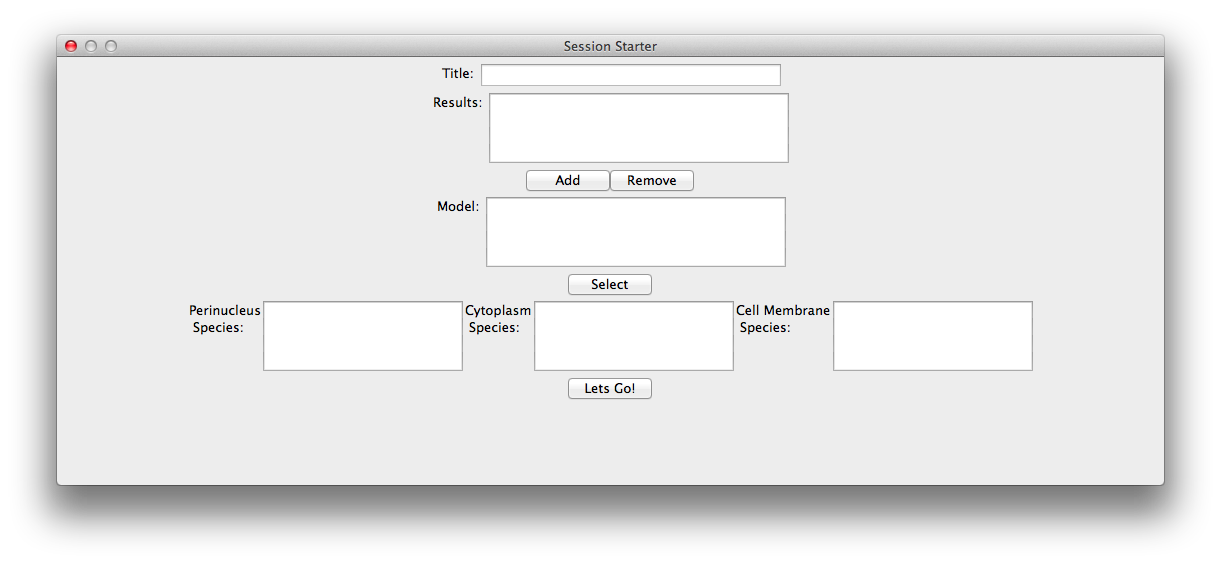
\includegraphics[height=0.5\textwidth]{images/old_wizard.png}
    \caption{Session dialogue, the precursor to the session wizard.}
    \label{fig:old_session_dialogue}
\end{figure}

The model viewer page in Figure~\ref{fig:page_4} is similar to the cell cross-sections used in Section~\ref{sec:animation}.  There are two drop down boxes.  These drop down boxes control what is displayed in the cell cross-section.  Species in files can be selected.  The cell cross-section displays which compartments in the cell the species is present in.  The compartments are parsed from the model file.  This means that the model file is a requirement for model viewing and cell level animation.  This cell cross-section has replaced the previous model visualisation.  The new model visualisation has two purposes. First, the user can sanity check that they have matching results and model files.  If a section of the cell has been left white then it acts as a cue to the user: if they were expecting the species to be present at that location then they know something has gone wrong.  Second, they can see how the model is structured.  The sections of the cell are labelled allowing the user to know what areas of the cell a species is present in.  This will hopefully increase their confidence with visualising and analysing the results from the models. Before the compartments were parsed from the model file automatically there was an user unfriendly system where the user had to input where in the cell a species is.  This was time consuming, difficult to use, and quite brittle.  At the time it assumed that there would be three compartments for every species, which is not a valid assumption.

\subsubsection{Collaboration}

It was not possible to perform an evaluation with any users of this feature.  Only one laptop was available for the evaluation sessions.  Although it is possible to run two instances of the program and start the collaboration feature, it is is not a representative demonstration as the two instances must be switched between and the changes are not seen in real time.

The evaluation of this feature has therefore been focussed on the responsiveness of the collaboration and the coverage of the functionality that can be collaborated on.

The implementation of real time collaboration is quite effective.  Almost all functionality that can be in a solo session has been implemented for collaborative work.  The only feature which cannot be used in the collaborative mode is the large plot. It was not possible to implement this feature because of the issue of closing the large plot dialogue.  The event that closes the dialogue would be the event that sends the message to the collaborator.  The collaborator would then have this method called.  There is then an infinite loop.  The displaying of a large version of the plot is a minor feature.  Not having access to it in the collaborative mode does not limit the user in their work.

The initial implementation of collaboration was not responsive enough.  It used blocking communication, effectively providing a lock around each action that effects the visualisation.  This involved waiting for a response from the collaborator to say that the change had been applied.  The \ac{UI} would be appear locked to the user for the duration of this message.  The collaboration features were only tested on internal networks where that duration would be minimal.  Even with minimal duration it was a frustrating experience being locked out of the \ac{UI}.  Communication to users across non internal networks could only be slower and therefore more frustrating to the user.  For this reason non blocking communication was implemented.  A thread is now created for each message sent.  This allows the \ac{UI} to not be locked out.  It did require losing the mutual exclusion guarantee.  This made the \ac{UI} more responsive, but sacrificed guaranteed correctness. Section~\ref{sec:ordering} discusses this further.

\subsubsection{Search Results}
\label{sec:search_eval}

Using plots as queries was a difficult feature to evaluate.  The ideal evaluation would have a large set of plots that were representative of the data generated by Bio-PEPA.  The set would have a subset of labelled similar plots.  We could then evaluate by using a plot, with known similar plots, as a query and seeing how many of the similar plots are ranked highly by \ac{tf.idf} weighted cosine.

In lieu of a real data set, an artificial set was used.  A random markovian walk was used to generate a corpus of time series data.  This corpus did not have a labelled set of similar plots, so similar plots were generated.  The query plot was taken and mutated in various fashions.  The mutations matched the criteria that were discussed in Section~\ref{sec:search}.  The similar plots generated through mutation can be seen in Appendix~\ref{sec:mutants}.

The experiments were run on this artificial corpus.  A number of experiments were performed:
\begin{itemize}
\item Experiment 1 -- One iteration of \ac{tf.idf} weighted cosine with 10000 plots and no labelled similar plots.  The purpose of this experiment was to see what would be returned as similar if no similar plots were defined.
\item Experiment 2 -- One iteration of \ac{tf.idf} weighted cosine with 10010 plots including 10 similar plots generated through mutation.  The purpose of this experiment was to see how many of the labelled similar plots are returned as being similar.
\item Experiment 3 -- 100 iterations of \ac{tf.idf} weighted cosine with 1010 plots in the corpus.  The purpose of this experiment was to repeat Experiment 2 with multiple iterations.
\item Experiment 4 -- 1000 iterations of \ac{tf.idf} weighted cosine with 110 plots in the corpus.  The purpose of this experiment was to repeat Experiment 2 with even more iterations than Experiment 3.
\end{itemize}

The results were extremely positive.  The findings from each experiment are discussed in detail below.

\paragraph*{Experiment 1:} The results from this experiment can be seen in Table~\ref{table:tab1}.  These results have discarded the match between the query and itself.  The table shows the top 10 most similar plots found by \ac{tf.idf} weighted cosine and the measure of their similarity.  The plots of these graphs can be seen in Appendix~\ref{sec:experiment1}.  We can see in some graphs, particularly Figure~\ref{fig:ex1_1} and Figure~\ref{fig:ex1_3}, that there are structural similarities between the query plot and the result plots.  In some other graphs, particularly Figure~\ref{fig:ex1_2} and Figure~\ref{fig:ex1_8}, this similarity is less obvious.  This could be an issue of scale that is not obvious to the human eye.  It could also be a failing in the method for determining similarity.

\begin{table}[h]
\begin{center}
    \resizebox{0.8\textwidth}{!} {\begin{minipage}{\textwidth}
    \begin{tabular}{ | l | c | c | c | c | c | c | c | c | c | c | }
        \hline
        Rank & 1 & 2 & 3 & 4 & 5 & 6 & 7 & 8 & 9 & 10 \\
        \hline
        line id & 256 & 7017 & 8341 & 1380 & 4997 & 5462 & 6648 & 2298 & 595 & 190 \\
        \hline
        similarity & 0.1804 & 0.1765 & 0.1629 & 0.1623 & 0.1608 & 0.1601 & 0.1584 & 0.1575 & 0.1566 & 0.1562 \\
        \hline
    \end{tabular}
    \caption{10 most similar plots from Experiment 1}
    \label{table:tab1}
    \end{minipage}}
\end{center}
\end{table}

\paragraph*{Experiment 2:} The results of this experiment can be seen in Table~\ref{table:tab2}.  The results have discarded the match between the query and itself.  The table shows the top 10 most similar plots found by \ac{tf.idf} weighted cosine and the measure of their similarity.  This experiment contained the 10 mutated similar plots.  The 10 mutated plots are the entirety of the top 10.  Applying \ac{tf.idf} to Lin and Li's work~\cite{structural_similarity} appears to have been justified.  The three plots that were purely scalings of the original data have been returned as identical.  This is the correct behaviour of the algorithm as it is a scale invariant algorithm.  The eleventh most similar plot was plot 256, which was the most similar in Experiment 1.

\begin{table}[h]
\begin{center}
    \resizebox{0.8\textwidth}{!} {\begin{minipage}{\textwidth}
    \begin{tabular}{ | l | c | c | c | c | c | c | c | c | c | c | }
        \hline
        Rank & 1 & 2 & 3 & 4 & 5 & 6 & 7 & 8 & 9 & 10 \\
        \hline
        line id & 10002 & 10001 & 10000 & 10003 & 10008 & 10009 & 10005 & 10004 & 10007 & 100006 \\
        \hline
        similarity & 1.0 & 1.0 & 1.0 & 0.8980 & 0.8902 & 0.8525 & 0.8349 & 0.7787 & 0.7086 & 0.6649 \\
        \hline
    \end{tabular}
    \caption{10 most similar plots from Experiment 2}
    \label{table:tab2}
    \end{minipage}}
\end{center}
\end{table}

\paragraph*{Experiment 3:} In all 100 experiments the top ten most similar plots found by \ac{tf.idf} weighted cosine, excluding the query itself, were the mutated similar plots.  This is a positive indication that the approach for determining similarity was a valid one.  It does, however, indicate that using artificial data may have drawbacks.
\paragraph*{Experiment 4:} In all 1000 experiments the top ten most similar plots found by \ac{tf.idf} weighted cosine, excluding the query itself, were the mutated similar plots.  This is a positive indication that the approach for determining similarity was a valid one.  It does, however, indicate that using artificial data may have drawbacks.

\paragraph*{Findings:} The evaluation technique does have its limitations.  The data is artificial and may differ significantly from real data.  This was unavoidable as there was not enough real data to compare it to.  The experiments with multiple iterations were limited in how many plots could be included in the corpus.  The generation of the plots was a very computationally intensive process and limited the amount of data that could generated for experimentation.

The mutations used for defining similarity are quite clean operations.  In reality the similar plots would likely be fuzzier matches than were used in this experimentation.  This would require actual data to investigate.  This has possibly affected the results, especially in Experiments 3 and 4.

Despite the limitations of the evaluation technique, the results of the experiments showed great promise for this feature.  The results justified the inclusion of the feature and indicated that further investigation would be worth while.

\subsubsection{Animation}

Animation of cell cross-sections requires the model file to be provided.  Ideally the user would just need to provide the results file, but the results file does not include all the necessary information.  It was felt to be more user friendly to require the model file than having the user enter a lot of information by hand.

Users can use the model viewer, in the session wizard (Figure~\ref{fig:page_4}), to preview animation.  Once a session has been started the animation toolbar is made available.  The toolbar contains a play/pause button.  This enables discovery of two features.  The line drawn on the graph indicating current time and the time slider.  While the animation is playing the user can see the time slider and the line moving.  This provides a cue to them that they can move the slider to control time.

The species/file selectors and the button to switch between file-focussed and species-focussed modes are less obvious in their behaviour.  Users were unable to work out what these features did.  After having the features explained they were comfortable with them.  Discoverability was the issue with these features.  A solution was not found. User documentation would be a fix for this.

The appearance of the time slider in the \ac{UI} is a particular weak point in the \ac{UI}.  Many attempts were made to stretch the appearance of the slider widget but these were fruitless.

The performance of the animation was more than adequate.  The animation of the cell segments is very smooth.  The animation of the line on the graph is also fairly smooth, although choppiness in frame transitions has been noticed.  The performance is better than the usual plotting speed of the graph. This is because only a select part of the graph is being redrawn -- the vertical line.

Feedback from the users has been very positive for the animation feature.  It meets the goal of providing visualisations more familiar to the users.

\subsubsection{Annotation}

Annotation of the graph and the animation had to be implemented separately.  They also have to be evaluated separately.  One of the flaws of the current annotation implementation is the separation between the different annotations.  This is not user friendly as they have to learn two different systems, each with different behaviours.

\paragraph*{Annotation of the Graph:} Placing annotations is now quite user friendly.  The annotation type is chosen from the toolbar and then the graph is clicked to place the annotation.  Arrow annotations have an arrow that follows the mouse allowing the user to see the appearance before placing the annotation.  This was not possible for the text and circle annotations.

Selecting annotations is not user friendly enough.  The need to right click to select an annotation is assumed knowledge.  It has not been made obvious enough to the user.  No user was able to initiate the context menu without being told about it.  No solution was implemented.  One fix would be to remove the right click aspect, and instead use a hover menu.

Editing text and deleting provide the user with control over the annotation. More control needs to be provided in the future, in particular the ability to move annotations.

\paragraph*{Annotation of the Animation:} Placing annotations is reasonably user friendly.  The dialogue acts as a guide to the user.  Having to click on a cell cross-section to place the annotation was hoped to be obvious as it follows the same behaviour as with the graph annotations.  This was not the case.  Text has been added to the dialogue to make this more obvious.

There is also too much of a disconnect between the animation panel and the panel containing the list of annotation.  This was felt necessary due to space constraints.  A more desirable approach would be similar to the graph annotations which are handled entirely from the toolbar, not a separate panel on the \ac{UI}.

\subsubsection{Normalisation and Export}

This is quite a user friendly feature.  This has been evidenced by the users having no trouble with the feature.  Normalising the data uses a checkbox menu item to toggle on or off.  This provides a visual clue to the user that it is a toggle-able state.  It should indicate as well that if they press the menu item and do not like the results that they can press the menu item again and revert to the previous appearance.

Normalisation and export are both operations on the data and so have been grouped together on the menu.  The main issue with normalisation was how annotations should behave.  The approach was described in Section~\ref{sec:normalised}.  This was an adequate solution and keeps the state visible to the user.

\subsubsection{Performance}

The speed of the tool is not great.  It becomes sluggish in some situations.  This is mainly due to \texttt{matplotlib}.  \texttt{matplotlib} is the de facto standard for graphing in Python. This, amongst other reasons (detailed in the MPP report), led to it being chosen for the graph visualisations in the project.  When features such as plotting the intensity of the gradient were added, \texttt{matplotlib} was pushed to its limits as it was being asked to plot thousands of lines.  It was discovered that \texttt{matplotlib} is not optimised for speed, it is instead optimised for producing graphs of a publishable standard.  This poses a dilemma: researchers want to be able to generate quality graphs, whilst the tool wants to offer real time interactivity and customisation.  There are tweaks that can be applied to make \texttt{matplotlib} faster. There are also alternative graphing libraries that could be considered.  Threading was also looked into but caused segmentation faults.

\subsection{Testing and Logging}

The development of the project involved little formal testing and logging.  The intention had been to develop tests, but these tests never came to fruition.  The development work was too tempting. The lack of tests caused problems later in development.  New features being implemented, which would often involve refactoring, would sometimes break existing functionality.  These bugs might then not be discovered until the next round of user testing.  This was not what the users wanted to be presented with.  Having tests would potentially have revealed these bugs.

Another oversight was the lack of logging in the program.  This only became a problem towards the end of the project as it got more complex.  It would, sometimes, be difficult to recreate a bug that the users had discovered.  This made the bug harder to fix.  The problem reached its peak during the implementation of real time collaboration.  Trying to debug the distributed communication without formal logging was challenging.  Print statements were used as a simple form of logging that was somewhat helpful.  Having a more structured logging framework in place from the start would have eased debugging throughout the development process.



